%Autor: Gianluca Picciola
%Projekt 4, EIT 2018

\documentclass{fhnwreport}

\usepackage{pdflscape}%Für Querformat
\usepackage[T1]{fontenc}
\usepackage{trfsigns} %Benutzung Mathematische Zeichen
\usepackage{textgreek}
\renewcommand{\figurename}{Fig.}
\usepackage{float}
\usepackage{pdfpages}%Import von PDF
\usepackage{dsfont}
\usepackage{ngerman}
\usepackage{amsmath}
\usepackage{subfigure}
\usepackage[utf8]{inputenc}
\usepackage{cancel}%zum durchsteichen
\usepackage{polynom}%zur polynomdivision
\usepackage{fancyhdr}%für Kopfzeile
\usepackage{listings}
\usepackage{geometry}
\usepackage{paralist}
\usepackage{nameref}%Referenz
\usepackage{cite}%Quellen
\usepackage{graphicx}
\graphicspath{ {Data/} }
\bibliographystyle{IEEEtran}
\usepackage{booktabs}
\usepackage{tikz}
\usepackage{amsmath}
\usetikzlibrary{arrows}
\usepackage{lmodern}  
\usepackage{wrapfig} 
\usepackage{siunitx}
\DeclareSIUnit \Volt {V} 
\usepackage[normalem]{ulem}
\useunder{\uline}{\ul}{}

\setcounter{tocdepth}{2} % Set depth of table of contents
\setcounter{secnumdepth}{3}


\title{%
  Fachbericht\\[2ex]
  Dojo}
\author{%
  Team 5, FS 18}

\begin{document}

% Titel
\maketitle

\vfill

% Titelbild
\begin{figure}[H]
	\centering
	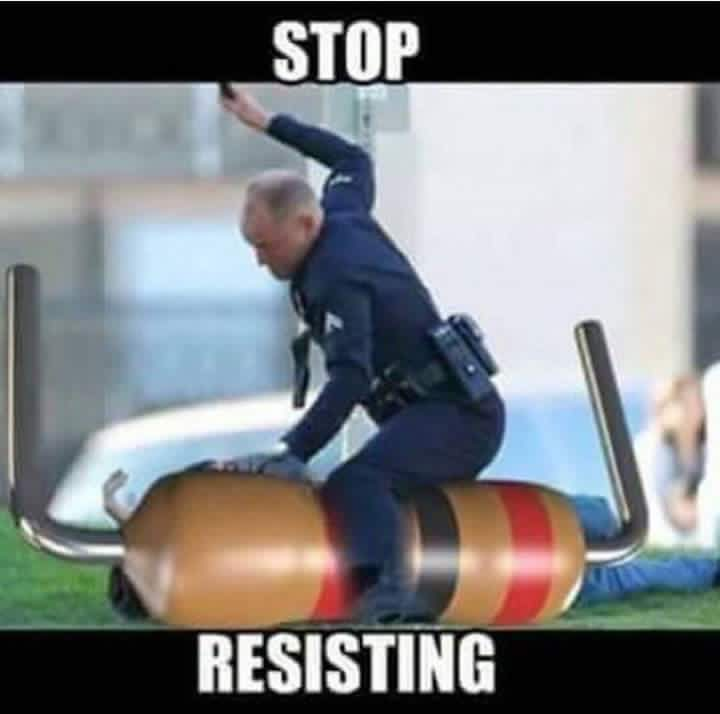
\includegraphics[width = 0.5\textwidth]{Data/Titelbild}
	\label{fig:Titelbild}
\end{figure}

\vfill

\begin{tabbing}
Auftraggeber: \hspace{2em} \=  Gysin Hans, Kalbermatter Jana \\[2ex]
Betreuer:  \>  Meier Matthias, Schleuniger Pascal, Gertiser Anita, \\ \> Domenghino Bonny, Dubach Roswitha \\[2ex]
Team:  \> Zoller Simon \\ 
\> Hunziker Severin \\
\> Loosli Lukas \\
\> Picciola Gianluca \\
\> von Däniken Elias \\
\> Giambonini Joscha \\
\> Knupfer Mischa \\[2ex]
Studiengang: \> Elektro- und Informationstechnik
\end{tabbing}

\hbox{}
\clearpage


%%%%%%%%%%%%%%%%%%%Abstract%%%%%%%%%%%%%%%%%%%%%%%

%Durch den Stern wird die Nummerierung unterdrückt, also nur fett geschrieben.
\section*{Abstract}

Abstract Abstract Abstract

\newpage

%%%%%%%%%%%%%Inhaltsverzeichnis%%%%%%%%%%%%%%%%%%%

\tableofcontents
\newpage

%%%%%%%%%%%%%%%%%%%%%%%%%%%%%%%%%%%%%%%%%%%%%%%%%%






%%Hier werden die einzelnen Dokumente eingefügt%%%

%%%%%%%%%%%%%%%%%Einleitung%%%%%%%%%%%%%%%%%%%%%%%

% !TEX root = Fachbericht.tex
\section{Einleitung} \label{sec:einleitung}
Einführung in das heikle Thema Museen in der Schweiz. Die Revolution durch Dojo.

%%%%%%%%%%%%%%%%%%Grundlagen%%%%%%%%%%%%%%%%%%%%%%

% !TEX root = Fachbericht.tex
\section{Grundlagen} \label{sec:grundlagen}
Hier werden die wichtigsten Grundlagen zusammengefasst und erläutert.
% !TEX root = Fachbericht.tex

%Verwendet die hier aufgeführten Beispiele damit keine Probleme entstehen.

%section  = 3.Hardware
%subsection = 3.1 Hardware
%subsubsection = 3.1.1 Hardware
%wird ein Stern angefügt, erscheint keine Nummerierung und die Auflistung im Inhaltsverzeichnis wird unterdrückt



\subsection{Beispielabschnitt} \label{sec:beispielabschnitt}

%Beispiel für das Einfügen eines Bildes, inklusive der Beschriftungen und falls nötig Quellenverweis: 
%Achtung: \caption[Steht im Abbildungsverzeichnis]{unter dem Bild}
%\label{fig: als Referenz für spätere Verweise, gewählter Name erscheint}
%Vorsicht: das Bild muss exakt die gleiche Beschriftung im Dateinamen haben, wie im Pfad Data/Spannungsnetzebenen, sonst funktioniert es nicht.

\begin{figure}[htbp]
\centering
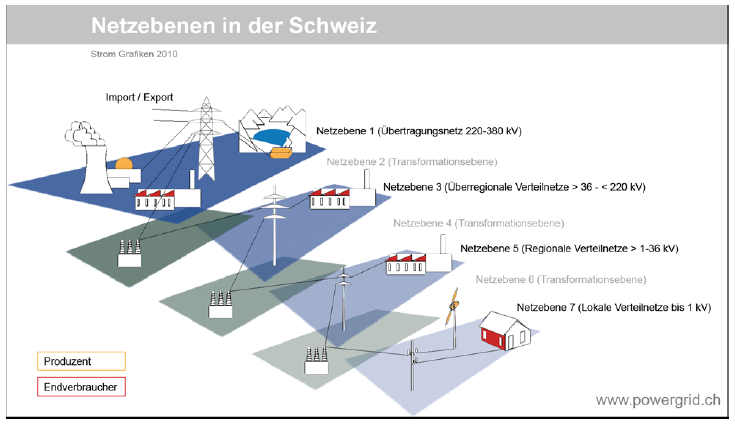
\includegraphics[width=1\textwidth]{Data/Spannungsnetzebenen}
\caption[Netzebenen\cite{eetgl_skript}]{Netzebenen}
\label{fig:Netzebenen}
\end{figure} 

%2 Beispiele für Formeln:

So kann aus den Dokumenten \cite{Niklaus_Skript}, \cite{ant_skript}, \cite{dt1_skript}, \cite{eetgl_skript}, \cite{mc1_skript} und \cite{INA_128} entnommen werden, dass die folgenden Beziehungen korrekt sind:

\begin{equation}
\centering
u(t) = \^{U} \cdot \cos (\omega t + \varphi u)
\label{eq:Spannungsfunktion}
\end{equation}

\begin{equation}
\centering
U = U_{eff} = \sqrt{\dfrac{1}{T}\cdot \int_0^T u^2(t) dt}
\label{eq:Effektivwert}
\end{equation}

Anschliessend kann im Text der Verweis gemacht werden. Mit der Gleichung \ref{eq:Spannungsfunktion} und \ref{eq:Effektivwert} wird die Abbildung \ref{fig:Netzebenen} selbsterklärend. Ebenfalls kann auf das Kapitel \ref{sec:grundlagen} verwiesen werden. Noch zwei Beispiele mit Tabelle \ref{tab:BelasteteMessung} und \ref{tab:SpannungsmessungTabelle}. Es gibt auch einen Tabellengenerator für LATEX, sowie das Programm JabRef, mit welchem bereits der entsprechende Code für das bibtex-file quelle erstellt.

\begin{table}[htbp]
\centering
\begin{tabular}{lllllllllll}
\multicolumn{3}{c}{\textbf{Wattmeter}}                       & \textbf{} & \multicolumn{3}{c}{\textbf{Projekt}}                         & \textbf{} & \multicolumn{3}{c}{\textbf{Abweichung}}                         \\
\textbf{P {[}W{]}} & \textbf{U {[}V{]}} & \textbf{I {[}A{]}} & \textbf{} & \textbf{P {[}W{]}} & \textbf{U {[}V{]}} & \textbf{I {[}A{]}} & \textbf{} & \textbf{P {[}\%{]}} & \textbf{U {[}\%{]}} & \textbf{I {[}\%{]}} \\ \cline{1-3} \cline{5-7} \cline{9-11} 
5.48             & 230.7             & 0.024              &           & 5.00             & 230.58             & 0.0328              &           & 8.7                & 0.05                & 36.6                \\
8.63              & 230.6             & 0.0377              &           & 8.00              & 230.34             & 0.0376              &           & 7.3                & 0.11                & 0.27                \\
73.72              & 235.90             & 0.312              &           & 72.00              & 235.04             & 0.312              &           & 2.33                & 0.36                & 0.10                \\
117.30             & 236.60             & 0.497              &           & 115.88             & 235.77             & 0.494              &           & 1.21                & 0.35                & 0.52                \\
130.80             & 236.10             & 0.556              &           & 129.60             & 235.35             & 0.554              &           & 0.92                & 0.32                & 0.50                \\
                   &                    &                    &           &                    &                    &                    &           &                     &                     &                     \\
150.30             & 236.00             & 0.639              &           & 149.61             & 235.83             & 0.637              &           & 0.46                & 0.07                & 0.20                \\
203.30             & 236.10             & 0.860              &           & 202.19             & 236.21             & 0.861              &           & 0.55                & 0.05               & 0.07               \\
303.50             & 235.30             & 1.291              &           & 302.00             & 235.70             & 1.289              &           & 0.49                & 0.17               & 0.19                \\
493.70             & 235.00             & 2.100              &           & 493.48             & 235.87             & 2.107              &           & 0.04                & 0.37               & 0.35               \\
724.60             & 234.20             & 3.060              &           & 725.43             & 235.56             & 3.100              &           & 0.11               & 0.58               & 1.31               \\
                   &                    &                    &           &                    &                    &                    &           &                     &                     &                     \\
395.20             & 235.60             & 4.132              &           & 420.93             & 236.13             & 4.114              &           & 6.51               & 0.22               & 0.43                \\
404.10             & 235.90             & 4.189              &           & 437.88             & 235.64             & 4.265              &           & 8.36               & 0.11                & 1.80               \\
1384.80            & 233.00             & 6.935              &           & 1409.02            & 234.96             & 6.930              &           & 1.75               & 0.84               & 0.06                \\
1595.40            & 232.00             & 7.057              &           & 1609.30            & 234.95             & 7.022              &           & 0.87               & 1.27               & 0.49                \\
1885.00            & 231.10             & 8.184              &           & 1899.96            & 234.40             & 8.162              &           & 0.79               & 1.43               & 0.27               
\end{tabular}
\caption{Belastungsmessung aufgelistet nach Messbereich}
\label{tab:BelasteteMessung}
\end{table}

\begin{table}[!htbp]
\centering
\begin{tabular}{lll}
\textbf{Multimeter V} & \textbf{Messung V} & \textbf{Abweichung \%}\\ \hline
100.5        & 102.75    & 2.2       \\
150.0        & 151.09    & 0.7       \\
199.5        & 199.88    & 0.2       \\
220.2        & 220.45    & 0.1       \\
230.5        & 230.77    & 0.1       \\
240.1        & 240.36    & 0.1       \\
           
\end{tabular}
\caption{Validierung der Spannungsmessung}
\label{tab:SpannungsmessungTabelle}
\end{table}

%%%%%%%%%%%%%%%%%%Hardware%%%%%%%%%%%%%%%%%%%%%%

% !TEX root = Fachbericht.tex
\section{Hardware} \label{sec:hardware}
Einführung in die Hardware. Hier müssen die wichtigsten Komponenten gezeigt werden. Anschliessend kann systematisch das Zusammenspiel und der komplette Aufbau detailliert erklärt werden.

%%%%%%%%%%%%%%%%Software%%%%%%%%%%%%%%%%%%%%%%%%%%

% !TEX root = Fachbericht.tex
\section{Software} \label{sec:software}

%%%%%%%%%%%%%%Validierung%%%%%%%%%%%%%

% !TEX root = Fachbericht.tex
\section{Validierung} \label{sec:validierung}


%%%%%%%%%%%%%%%%Kosten%%%%%%%%%%%%%%%%%%%%%%%

% !TEX root = Fachbericht.tex
\section{Kosten} \label{sec:kosten}
Die unten aufgeführte Tabelle zeigt eine Kostenaufstellung der verwendeten Bauteile.
\begin{table}[h]
\centering
\begin{tabular}{llll}
\textbf{Bezeichnung}   & \textbf{Art.Nr.} & \textbf{Menge} & \textbf{Preis}  \\
Mikrocontroller        & 110-38-920       & 1              & 39.60           \\
SD-Shield              & 110-81-045       & 1              & 17.90           \\
WiFi-Modul             & 300-74-914       & 1              & 27.40           \\
Shunt 10m              & 300-37-183       & 1              & 1.00            \\
Schaltnetzteil         & 512613-62        & 1              & 18.95           \\
Shunt 100m             & 300-37-198       & 1              & 0.91            \\
Shunt 200m             & 300-37-199       & 1              & 0.91            \\
Relais                 & 137-07-139       & 3              & 3.30            \\
Printklemme            & 148-38-692       & 6              & 0.86            \\
Sicherungshalter       & 300-43-424       & 3              & 0.33            \\
Schutzdiode 400V       & 170-13-536       & 1              & 0.60            \\
MOSFET                 & 171-03-872       & 3              & 0.10            \\
Z Diode                & 170-30-380       & 3              & 0.06            \\
Operationsverstärker   & 173-01-406       & 1              & 0.55            \\
Chargepump             & 173-27-081       & 1              & 3.15            \\
Diode                  & 300-41-120       & 3              & 0.15            \\
Anschlussstecker       & 110-73-283       & 1              & 9.95            \\
Anschlussstecker       & 143-49-992       & 1              & 1.40            \\
Spannungsreferenz 5V   & 300-19-461       & 1              & 0.50            \\
Spannungsreferenz 2.5V & 173-28-504       & 1              & 1.84            \\
Kabel                  & 300-38-525       & 1              & 6.70            \\
Instrumentenverstärker & 173-38-189       & 3              & 8.30            \\
Kunststoffbolzen       & 148-43-081       & 4              & 0.67            \\
Kunststoffmutter       & 148-50-020       & 4              & 0.08            \\
Gehäuse                & 300-64-369       & 1              & 8.30            \\
SD Karte                          & 173-81-870          & 1              & 4.75               \\
Widerstände                       & Diverse          &                & 3.00            \\
Kondensatoren             & Diverse          &                & 3.00            \\
                       &                  &                &                 \\
\textbf{Gesamtpreis}   &                  &                & \textbf{195.30}
\end{tabular}
\caption{Kostenzusammenstellung}
\label{tab:kosten}
\end{table}


%%%%%%%%%%%%%%%%Schlusswort%%%%%%%%%%%%%%%%%%%%%%%

% !TEX root = Fachbericht.tex
\section{Schlusswort} \label{sec:schlusswort}


%%%%%%%%%%%%%Ehrlichkeitserklärung%%%%%%%%%%%%%%%%

% !TEX root = Fachbericht.tex
\section{Ehrlichkeitserklärung} \label{sec:ehrlichkeitserklärung}
Der Projektleiter bestätigt mit der Unterschrift, dass der Bericht selbst verfasst und alle Quellen sauber und korrekt deklariert wurden.\\
\\
\\


\begin{tabular}{lp{22em}l}
 \hspace{3cm}   && \hspace{3cm} \\\cline{1-1}\cline{3-3}
 Ort, Datum     && Simon Zoller
\end{tabular}

\newpage

%%%%%%%%%%%Quellenverzeichnis mit Bibtex%%%%%%%%%%
\newpage
\section{Literaturverzeichnis}
\bibliography{quelle}

%%%%%%%%%%%%%%%%Abbildungsverzeichnis%%%%%%%%%%%%%%
\newpage
\section{Abbildungsverzeichnis}
\renewcommand{\listfigurename}{}
\listoffigures

%%%%%%%%%%%%%%%%Anhang%%%%%%%%%%%%%%%%%%%%%%%%%%%%
\newpage
\begin{appendix}
% !TEX root = Fachbericht.tex
\section{Anhang}
\subsection{Messbereiche}

\begin{figure}[htbp]
\centering
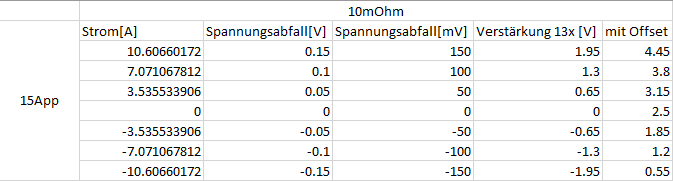
\includegraphics[width=0.8\textwidth]{Data/Tabelle10mOhm}
\label{fig:Tabelle10mOhm}
\caption[Messbereich 10m$\Omega$]{Messbereich 10m$\Omega$}
\end{figure}



\end{appendix}


%%%%%%%%%%%%%%%%Dokumentende%%%%%%%%%%%%%%%%%%%%%%
\end{document}